\documentclass{standalone}
\begin{document}
	
	\section{Accuracy}
	
	
	In this section I will discuss the pipeline segmentation compared with the annotations. 
	The pipeline was trained over $10$ CT scans, carefully selected from the three available datasets. This ensure a balanced cluster representation. 
	Using this set of centroids I have segmented the CT scans of the $3$ available datasets, and match the  achieved results whit the annotations, when available.
	
	The automatic pipeline was run on the servers of the Department of Physics and Astronomy (DIFA), and its able to achieve a segmentation in less than $2$ minutes. 
	
	\begin{figure}[h!]
		\centering 
			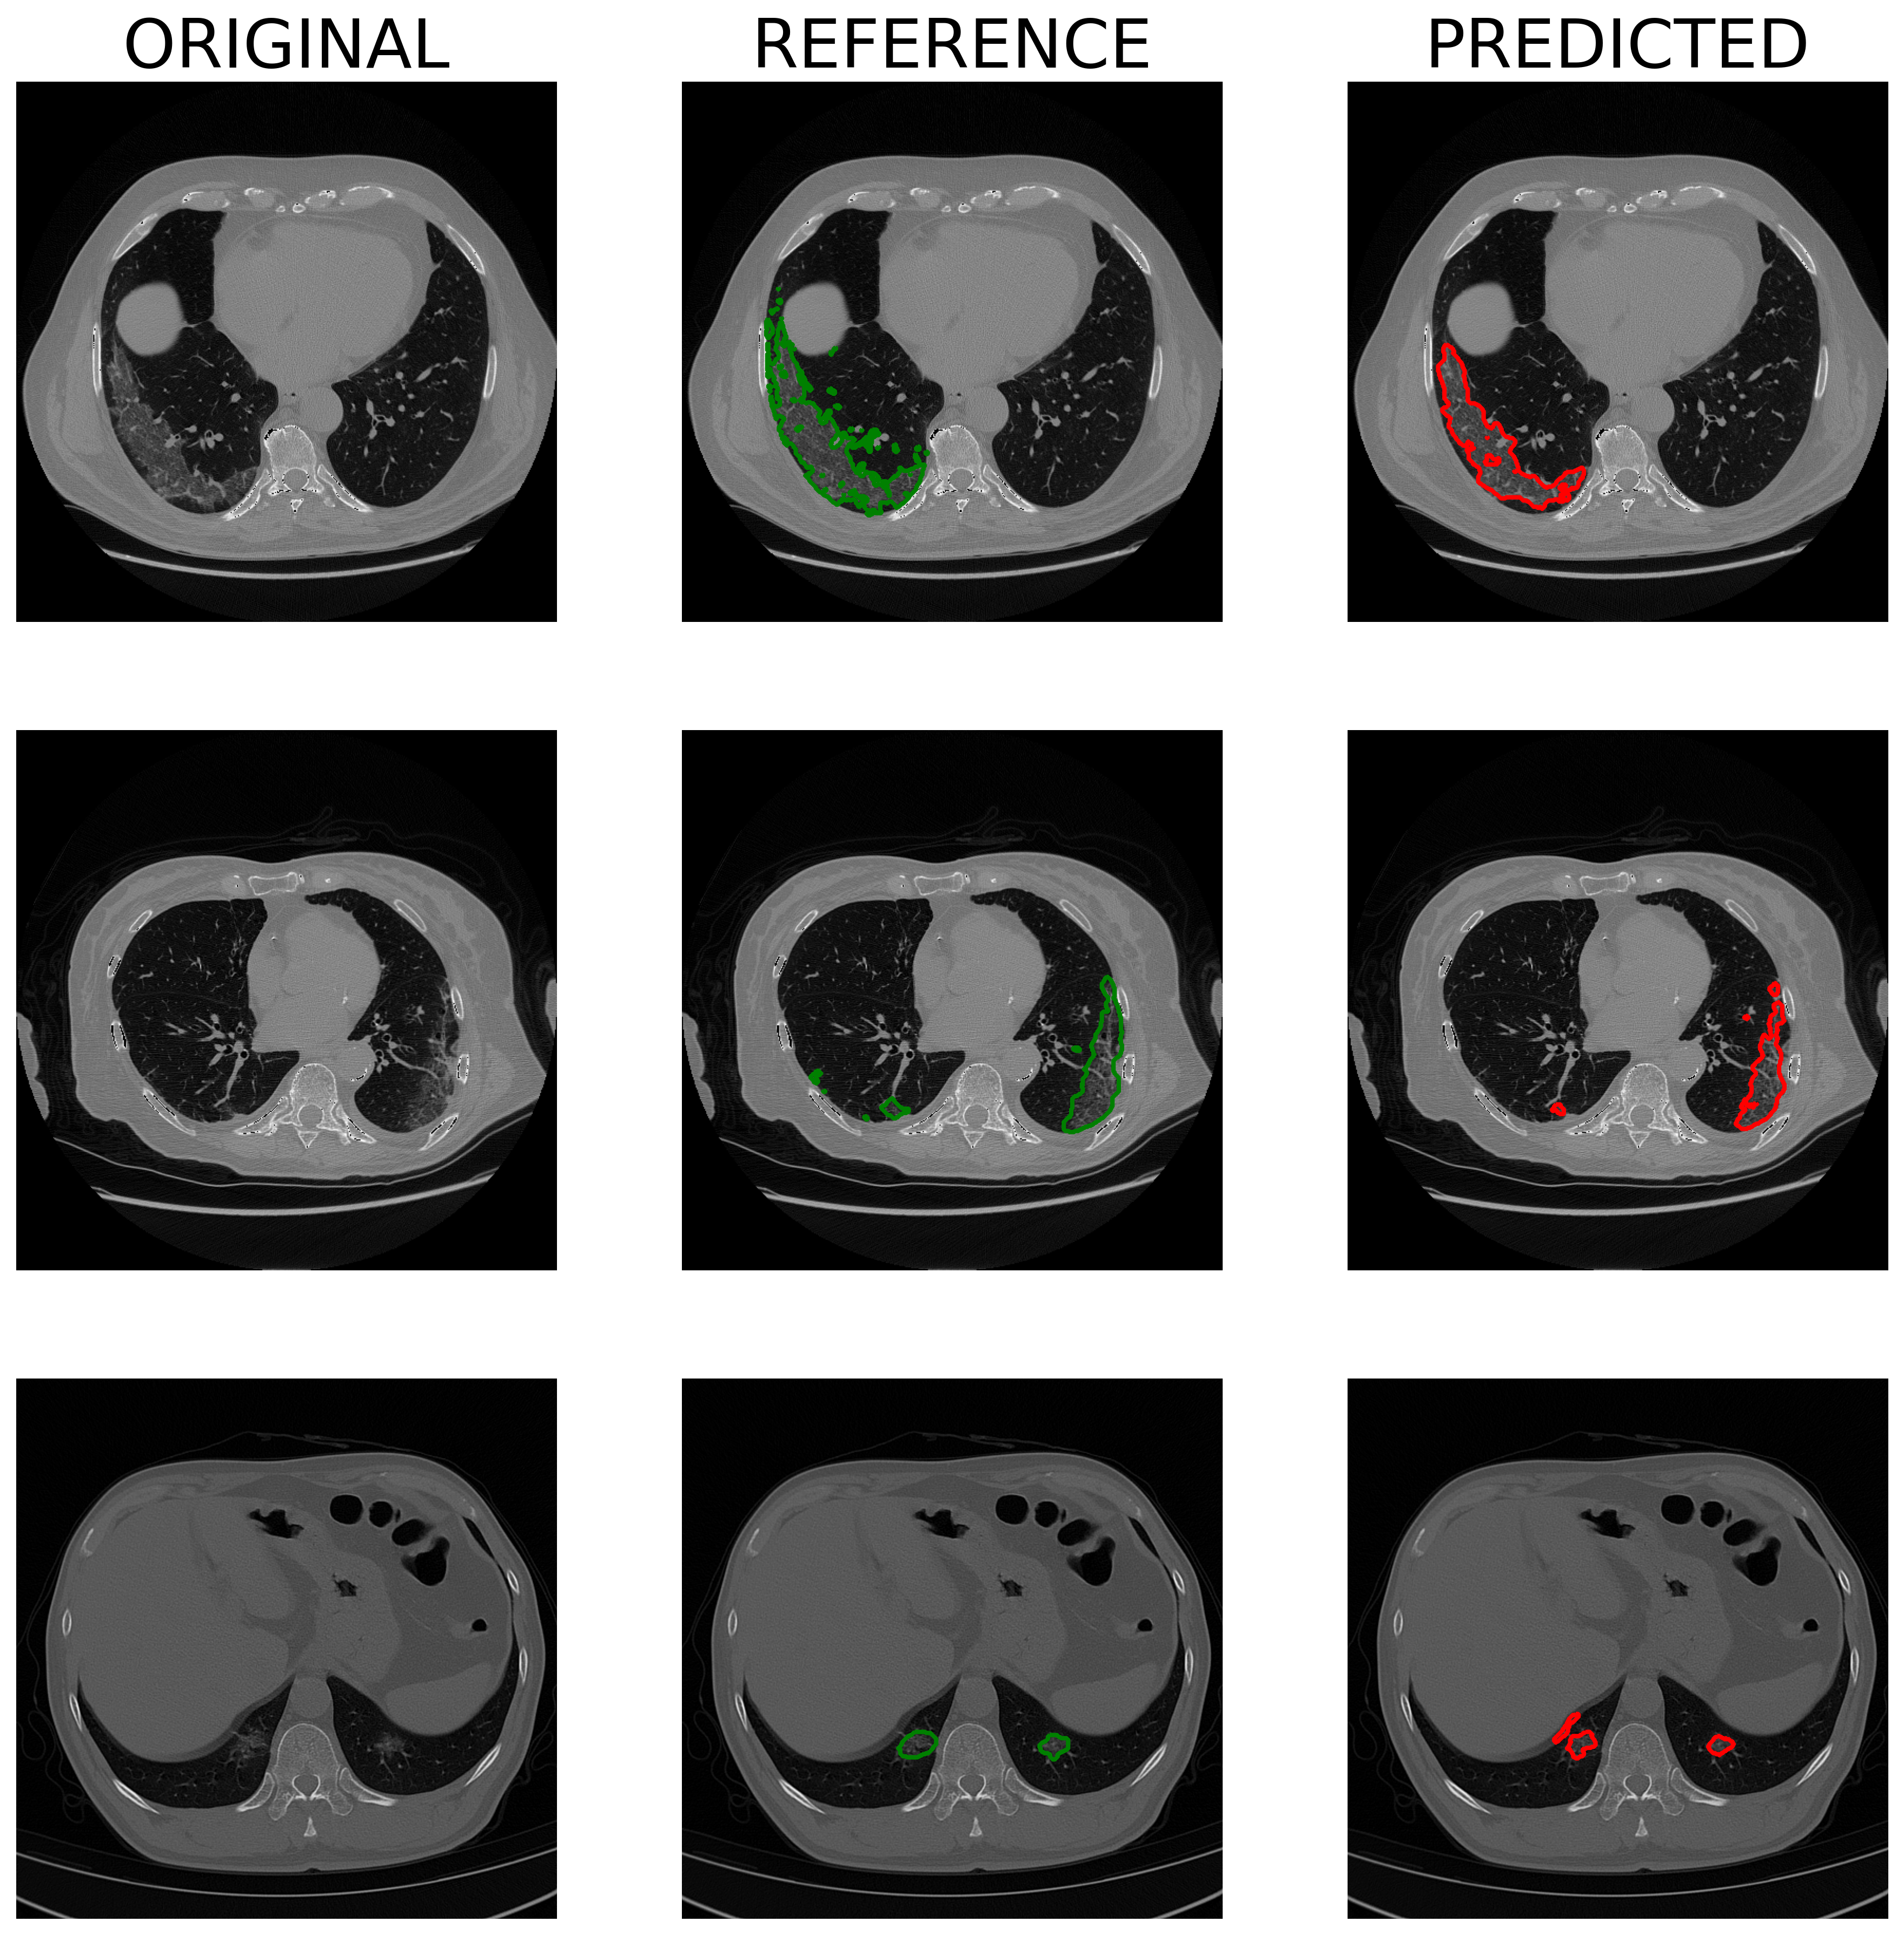
\includegraphics[scale=.2]{Results1.png}
			\caption{Comparison between the achieved segmentation (red) and the reference (green). We clearly see that the GGO ans CS areas are well identified and segmentented}\label{fig:Results}
	\end{figure}

	In \figurename\,\ref{fig:Results} I've reported a comparison between the achieved results and the reference segmentation. We an observe that GGO and CS areas are correctly segmented. 
	
	\begin{figure}[h!]
		\centering
			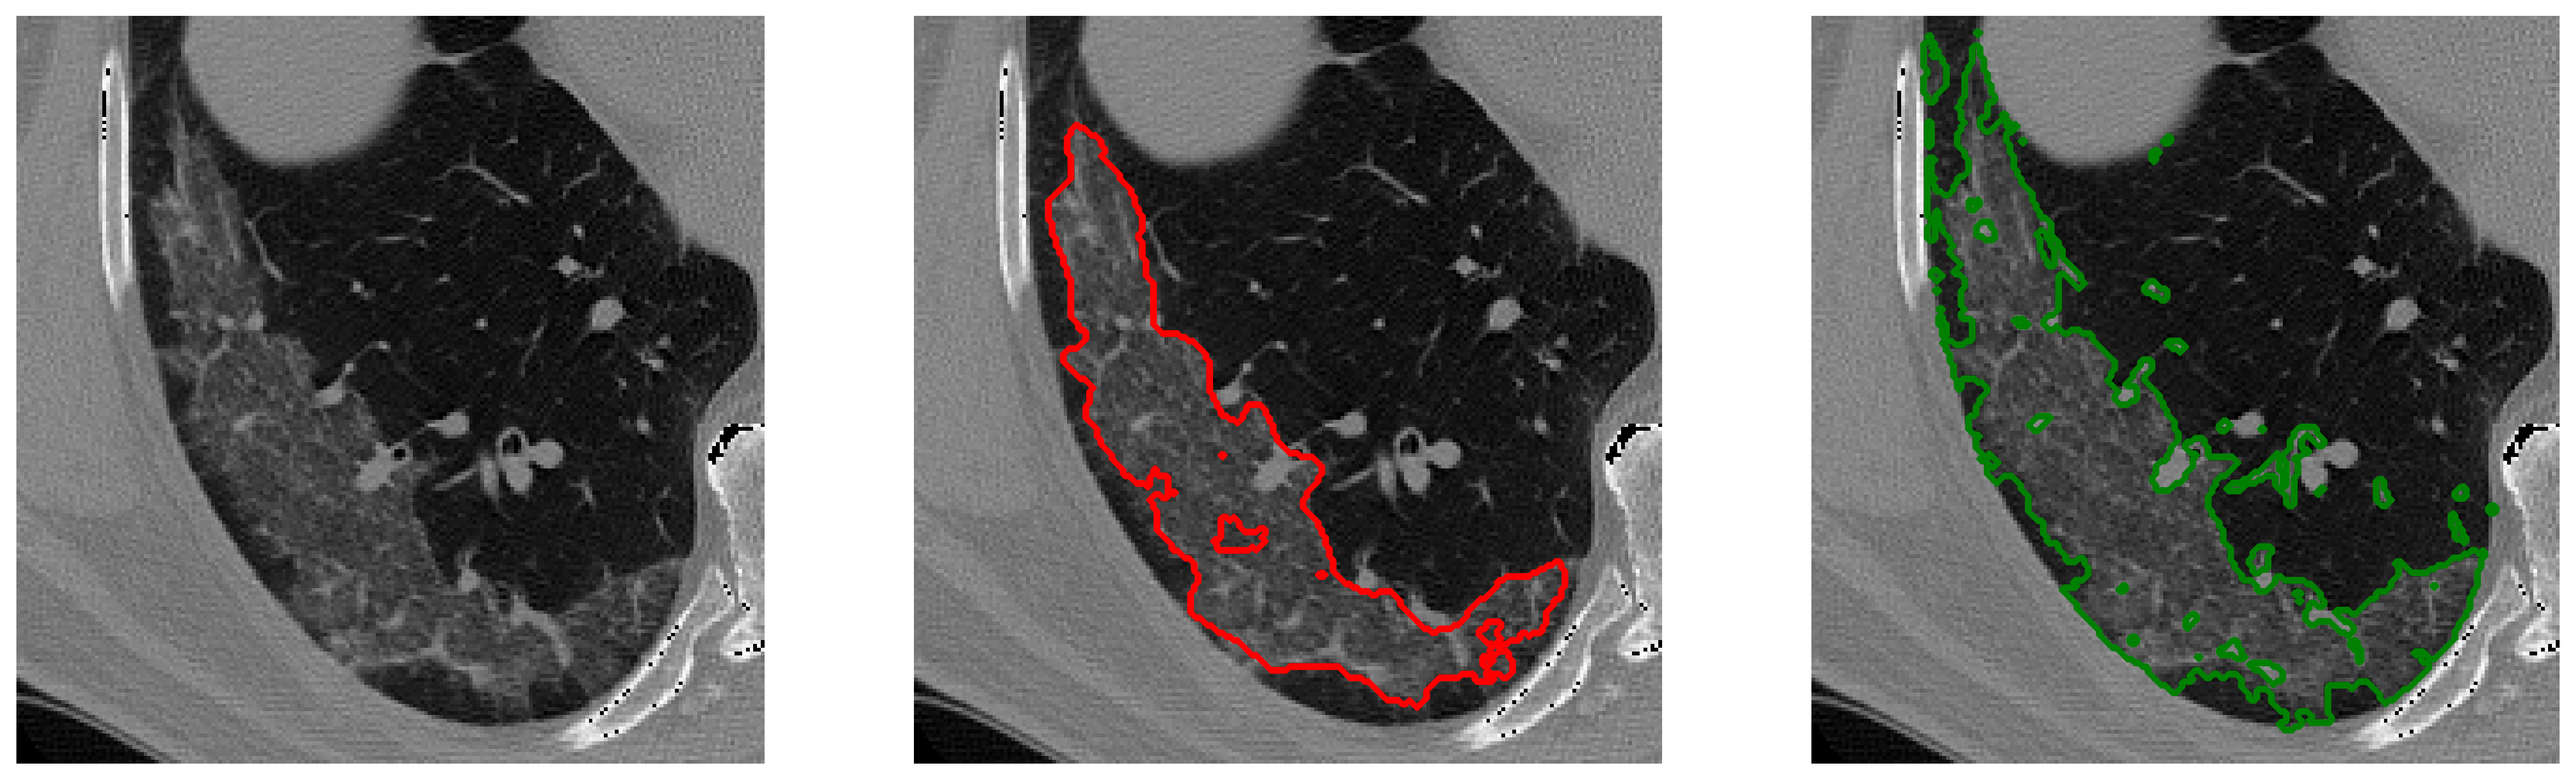
\includegraphics[scale=.37]{zoom.png}
			\caption{Focus on lesion area. From left to right we can observe the original image, the predicted lesion areas and the reference one. We can observe that the annotation  identify a larger area. The annotation identify also some spots outside the lesions which seems to be healthy tissue}\label{fig:zoom}
	\end{figure}
	
	
	In \figurename\,\ref{fig:zoom} I have reported a zoom on the identified lesions areas. As we can see both the pipeline segmentation and the annotations correctly identify the areas of interest. We can observe that in the semi-automatic method there are some spot which do not seem to belong to a lesion area. Moreover the automatic segmentation seems to identify a lesions with less areas.
	
	
	In \figurename\,\ref{fig:3Dlabel} I've reported a 3D rendering of the lung, with the identified lesions. In pink we can see the manual annotation, in green the segmentation achieved by the pipeline. From these images is more clear that the total estimated volume is different between the two methods. In particular the annotations incorporates a larger volume than the pipeline segmentation.
	
	\begin{figure}[h!]
	
		\centering 
			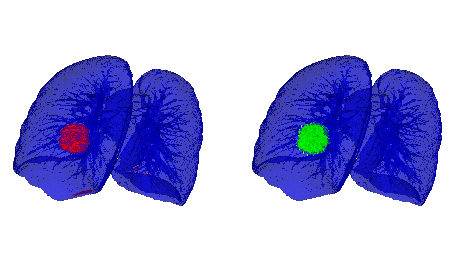
\includegraphics[scale=.4]{3Dlesion.png}
			\caption{3D representation of lesions. From left to right the manual annotation (pink) and the pipeline segmentation (green). We can observe that the segmented size of the area is different.}\label{fig:3Dlabel}		
	\end{figure}
	
	
	In order to assess the quality of the achieved segmentation, I've used two different method. 
	
	First of all I've compared both the pipeline segmentation and the annotations with a gold standard. In this way I was able to measure the proportion of the areas correctly identified.
	
	After that the segmentation was submitted to five experts in order to made a blind evaluation, comparing the pipeline segmentation with the reference one.
	
	In the section below I will describe these kind of measures.
	
	
\end{document}